\section{Toolchain check}
A citation resolves through the vendored IEEEtran.bst~\cite{li2013}.
% src: build-test (placeholder, not a paper fact)
\begin{figure}[t]
\centering
\begin{tikzpicture}[->,>=Stealth,node distance=2.2cm,state/.style={draw,rounded corners,minimum width=1.4cm}]
\node[state] (a) {State A};
\node[state,right=of a] (b) {State B};
\draw (a) -- node[above]{\scriptsize event} (b);
\end{tikzpicture}
\caption{TikZ placeholder diagram.}
\end{figure}
\begin{figure}[t]
\centering
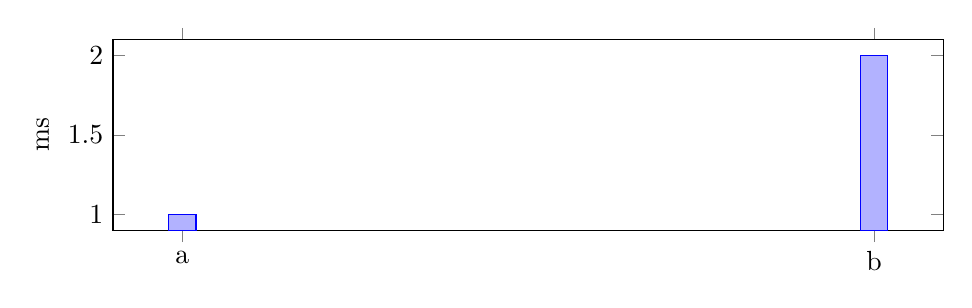
\begin{tikzpicture}
\begin{axis}[width=\columnwidth,height=4cm,ybar,symbolic x coords={a,b},xtick=data,ylabel={ms}]
\addplot coordinates {(a,1) (b,2)};
\end{axis}
\end{tikzpicture}
\caption{pgfplots placeholder plot (dummy data).}
\end{figure}
\begin{table}[t]
\caption{booktabs placeholder}
\centering
\begin{tabular}{lr}
\toprule
Item & Value \\
\midrule
x & 1 \\
\bottomrule
\end{tabular}
\end{table}
